\FrontmatterChapter{Abstract}
{\setlength{\parindent}{0pt}
\begin{Large}
\textbf{ARTIFICIAL VISION SYSTEM BASED ON A SYNTHETIC DATASET FOR A PICK AND PLACE APPLICATION}
\end{Large}

\textbf{Author: Ortiz de Zúñiga Mingot, Ignacio.} \\
Supervisors: Jesús López López, Álvaro \& Rodrigo Tobías, Ignacio de \\
Collaborating Entity: Grupo Antolin \\

\section*{Introduction}
The purpose of this project is the generation of a new artificial vision system for the recognition of parts for industrial use. This system will be implemented within a Grupo Antolín\textsuperscript{\textregistered} supply chain that will in turn feed an assembly and assembly line. The system must be able to identify multiple parts and determine the optimal grip point for each part. This is defined by its coordinates as well as the normal vector to the surface. In this way, a robotic arm with a gripping system by suction, suction cup or soft-robotics (varies depending on the piece to be picked up) will be able to collect them. The multitude of gripping tools as well as the need for a gripping point determination system is due to the great variety of existing pieces with a wide variety of shapes and sizes (1-30 cm).\\
\textbf{Key words:} Computer vision, Neural networks, Regressor, YOLO, Robotics, Assembly line

\section*{1. Project definition}
The objective of the project in collaboration with Grupo Antolin is the creation of a system capable of automating the process of preparing orders. The system will consist of vision systems and robotic arms responsible for making "baskets" with all the parts necessary to assemble an order, which will be assembled by an operator. Thanks to the automation of the generation of the "baskets", it is expected to be able to reduce the time needed to prepare the orders, thus improving the efficiency of the process. The entire process can be divided into several stages:

\begin{enumerate}
\item Order generation: depending on the demand and the customer's requirements, a list must be generated with all the necessary components for each order.
\item Structuring the order: The necessary parts are distributed in different sections and that is why an order must be created that determines the optimal parts collection order that reduces the collection time.
\item Collection of parts: This is an iterative process that must be carried out for each of the parts that make up the order.
\begin{enumerate}[label*=\arabic*.]
\item Offset to part. Depending on the configuration of the robot this system will vary, but the objective will always be the same. Move the robot to the region where the piece to be collected is located to be able to capture it and place it within the range region.
\item Part detection: applying detection algorithms, the part to be collected will be identified. Within the same area, numerous instances of the same part will be detected. You must choose the best-located piece/pieces with the greatest probability of success.
\item Grip point: after detecting the piece, it must be determined how the piece should be gripped. For this, the optimum grip point and the normal vector to said point must be determined.
\item Picking up the part: the necessary information is transferred to the robot so that it can pick up the part through the defined grip point. The gripping system to be used will depend on the type of piece.
\item Deposit and quality control: finally, the piece must be deposited inside the basket that constitutes the order. And through the artificial vision system, it must be verified that the desired piece has been correctly deposited in the basket.
\end{enumerate}
\item Quality control and traceability: before finalizing the order, it is analyzed one last time to verify that all the necessary parts are inside the basket. The order and all the necessary information for future traceability are registered in the system.
\item Transfer of the order: once the order is considered finished, it must be transferred to the assembly area to begin the assembly process.
\end{enumerate}

In this project, we will focus solely on the development of an artificial vision tool/system that will allow the detection of the piece as well as the definition of the gripping point and the normal vector to it. This system will be implemented to carry out stages 3.2 as well as 3.3. The system can also be used in stages 3.5 and 4 to carry out quality control and traceability tasks.

The system will be made up of two elements that will work in harmony. An image generator is capable of creating images of the pieces in a work environment as well as obtaining the necessary information on the position of each piece, the grip points, and their grip vectors. And an artificial vision system based on convolutional networks and a regressor for the prediction of the optimal grip point of each piece.

\section*{2. System description}
Due to the need to establish the optimal grip point for each piece, the system must grow in complexity, which implies that the dataset used must do so to the same extent. You want to have a large number of images for each piece with which you can train both YOLO and TINY YOLO. But in addition, you want to know for each of the regions marked for TINY YOLO you must know the coordinates of the grip point and its normal vector. Extracting this information manually is a complex and time-consuming process. Especially if it is considered that ideally thousands of instances of each piece should be obtained to train the neural networks.

For this reason, we have chosen to use an image generator based on the Blender rendering tool and the BlenderProc extension. The extension is a pipeline developed by DLR-RM in order to simplify the process of generating image datasets to train convolutional networks \citep{denninger2019blenderproc}. It is characterized by focusing on modularity by providing blender with the necessary tools to generate photorealistic scenes randomly but maintaining a modular structure that allows it to adapt to the problem.

With the help of BlenderProc an image generation system based on two parts has been created. In the first instance, two identical scenes are generated except for the exception of the parts used. The first image shows each of the pieces with their original textures. In the second, a piece with a modified texture is used with the insertion of QR codes that will later be used to extract the remaining information. The image generation process is shown below:

\begin{enumerate}
\item Scene: Loading the environment, parts, lighting, and camera. Throughout this process, randomness engines have been used so that the scenario, the type of pieces, and the number of pieces loaded are random. Finally, the camera is loaded and its hyperparameters are set to resemble the camera used during the tests.

\item Simulation: activation of the pieces so that they become part of the simulation and can interact with the environment, random positioning of the pieces, and physical simulation. In this way, it is possible to create random scenarios where the pieces are always in realistic positions and within the work area.

\item Rendering: settings for blender's output rendering and writing engines. The configuration used in this process will depend on the type of part present in the scene.
\end{enumerate}

Once the set of desired images has been generated, they must be processed to extract the necessary information and give the information a format that can be accepted and processed by neural networks. The post-processing process is divided into the following three stages:

\begin{itemize}
\item Position (YOLO): the first processing is characterized by being a simple transformation of the information generated by Blender and BlenderProc to a format that the neural network can understand. The transformation used consists of a change of origin of the position of the pieces and the elimination of the rest of the information that is not relevant to the problem.

\item Areas of interest (Tiny YOLO): the second processor must determine the possible grip areas for each piece. To do this, a cutout of each piece present in the image must be obtained for each image. And the position of the areas of interest of each clipping. To carry out this task, the Aruco library is going to be used, which is characterized by being able to detect QR codes with precision, speed, and efficiency.

\item Normal Vectors (Regressor): The objective is to obtain the normal vectors and the grip point for each piece. Therefore, the output, in this case, will be an individual image for each piece and a text file for each point of the piece. In this file, the centers of each point and the coordinates of its normal vector will be stored. The process for obtaining the image of each piece is identical to that of the areas of interest. This post-processing is characterized by the treatment of the normal image and the generation of text files with the information of each grip point.
\end{itemize}

\begin{figure}[ht]
	\centering
	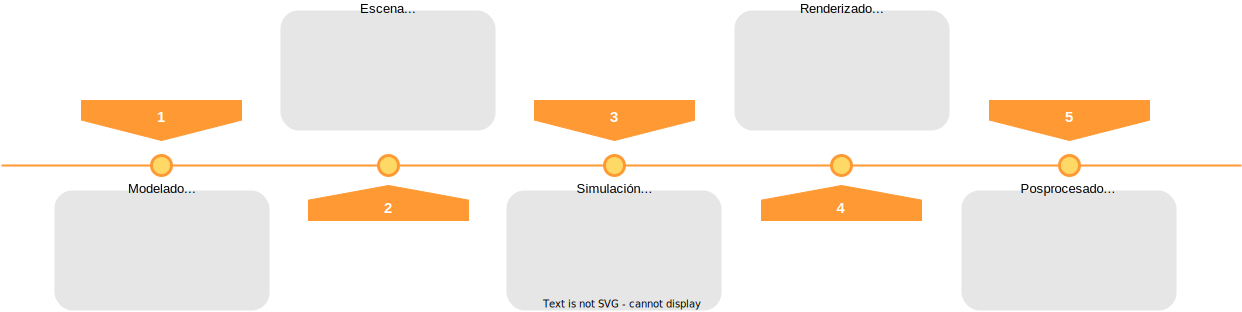
\includegraphics[width=0.9\textwidth]{Dataset/Arquitectura generador.pdf}
	\caption{Scheme of the system architecture}
	\label{chap:Abstract fig:Arquitectura generador}
	\vspace{-5pt}
\end{figure}

Once the dataset necessary to carry out this project has been developed, the developed solution can be introduced. Due to the complexity of the desired output (piece detection and gripping points), it has been necessary to develop a complex system made up of three neural networks:

\begin{itemize}
\item YOLO: This is the first neural network used and developed. It will be in charge of detecting the pieces within the work area and will be used as a basis to decide which piece should be collected. It is the only layer common to all the pieces.

To obtain the best possible results, it has been decided to use the YOLO evolutionary process. It is an iterative process in which, based on an objective function, the training hyperparameters are selected to optimize the training. These new hyperparameters are obtained through a genetic algorithm so that the best results of the previous iteration will be used as the basis for the creation of new hyperparameters. The objective function used is characterized by being a combination of $mAP@0.5$ with a contribution of 10\% and $mAP@0.5:0.95$ with a contribution of 90\%.

\begin{lstlisting}[language=Python]
 def fitness(x): 
     # Model fitness as a weighted combination of metrics 
     w = [0.0, 0.0, 0.1, 0.9]  # weights for [P, R, mAP@0.5, mAP@0.5:0.95] 
     return (x[:, :4] * w).sum(1) 
\end{lstlisting}

\item Tiny YOLO: A smaller and less powerful neural network but with more specialization. This network will be responsible for determining regions with possible grip points within the pieces (previously identified by YOLO). This second layer is specific to each piece and will only be applied to those pieces of high volume.

This second neural network must be trained as many times as pieces you want to introduce into the system. That is why the computational load must be reduced to avoid creating a slow and inefficient system. Fortunately, due to the great specialization of the network, it should only detect regions for one type of part, so the smaller version of YOLO can be used. The main advantage of YOLOv5 is the use of resources both at the computational and storage levels. The network occupies 4 MB and has a total of 1.9 million neurons. But despite its small size, it is capable of achieving surprising results capable of competing with powerful and heavy networks based on Fast-RCNN.

\item Regressor: This is the last layer of the artificial vision system. It is based on the output of Tiny YOLO and determines for each of the possible regions of interest the optimal grip point and its normal vector. This last layer is specific for each piece and will only be applied to those pieces of high volume.

The development of a neural network is a laborious process that requires multiple tests and attempts to develop a learning system in an optimized way. That is why multiple networks have had to be developed and trained to find an optimal system. The first step in network development has been to compare the impact of different network sizes. Networks with three, five, and seven convolutional layers have been compared to determine the number of layers needed to extract the features. Next, the impact of the size and depth of fully connected networks is analyzed. Next, different activation functions, different criteria, and optimizers are compared. It is observed in the results that the network suffers from overlearning, which is why dropout layers are finally implemented.
\end{itemize}

\begin{figure}[ht]
	\centering
	\includegraphics[width=0.5\textwidth]{Sistema de vision artificial/REGRESSION/CNNRegression.png}
	\caption{Scheme of the regressor}
	\label{chap:Abstract fig:Estructura Regresor}
\end{figure}

\begin{figure}[ht]
	\centering
	\includegraphics[width=0.8\textwidth]{Sistema de vision artificial/Diagrama_vision.png}
	\caption{Scheme of the artificial vision architecture}
	\label{chap:Abstract fig:Arquitectura sistema}
\end{figure}

\section*{3. Results}
As explained above, the system consists of two elements, the image generator, and the artificial vision system. And in turn, these are made up of multiple modules. But to analyze the behavior of these, they must be analyzed separately and as a whole.

The image generator must meet two requirements, the scenarios created must be random and the images must be photo realistic. The second objective is more than achieved thanks to the use of blender and high-quality texture maps. Therefore we must pay attention to maintaining randomness when creating the scenes. For this, three randomness engines have been used: NumPy, random, and uniformSO3 from Blenderproc. And all the engines are capable of generating uniformity, although it should be noted that uniformS03 will be used to generate the positions and when using Euler angles, a different distribution must be used.

\begin{figure}[ht]
	\ContinuedFloat
	\centering
	\begin{subfigure}[b]{0.3\linewidth}
		\includegraphics[width=\linewidth]{Dataset/Muestra_G1_a_sintetica.png}
	\end{subfigure}
	\begin{subfigure}[b]{0.3\linewidth}
		\includegraphics[width=\linewidth]{Dataset/Muestra_G3_sintetica.png}
	\end{subfigure}
	\begin{subfigure}[b]{0.3\linewidth}
		\includegraphics[width=\linewidth]{Dataset/Muestra_small_sintetica.png}
	\end{subfigure}
	\caption{Sample of images obtained using the image generator}
	\label{chap:Abstract fig:Muestras BlenderProc}
\end{figure}

\begin{figure}[ht]
	\ContinuedFloat
	\centering
	\begin{subfigure}[b]{0.3\linewidth}
		\includegraphics[width=\linewidth]{Dataset/numpy_uniform_histogram_1000.png}
	\end{subfigure}
	\begin{subfigure}[b]{0.3\linewidth}
		\includegraphics[width=\linewidth]{Dataset/random_choice_histogram_1000.png}
	\end{subfigure}
	\caption{Randomness of a uniform distribution generated by NumPy and Random}
	\label{chap:Abstract fig:numpy and random uniform}
	
	\begin{subfigure}[b]{0.3\linewidth}
		\includegraphics[width=\linewidth]{Dataset/blenderproc_uniformS03_histogram_1.png}
	\end{subfigure}
	\begin{subfigure}[b]{0.3\linewidth}
		\includegraphics[width=\linewidth]{Dataset/blenderproc_uniformS03_histogram_2.png}
	\end{subfigure}
	\begin{subfigure}[b]{0.3\linewidth}
		\includegraphics[width=\linewidth]{Dataset/blenderproc_uniformS03_histogram_3.png}
	\end{subfigure}
	\caption{Randomness of uniformSO3 from the BlenderProc package}
	\label{chap:Abstract fig:uniformS03}
\end{figure}

The second element that constitutes the system is the set of neural networks that make up the artificial vision system. As explained, it is made up of a total of three networks, and depending on the type of pieces, one or all of the networks will be used.

The first network to train is YOLO. Once the evolutionary process has been completed, two versions of YOLO have been trained with different hyperparameters. In both cases, it is observed how the neural network is capable of generalizing and extracting the information and characteristics of the pieces. But the lack of training is also observed as the metrics continue to improve when training was stopped. But despite this, you can see the great performance and capabilities of YOLO. A clear improvement is also observed when using the hyperparameters obtained by the evolutionary algorithm both in training and in validation.

Finally, the precision and validation recall has been obtained (see \autoref{chap:Artificial vision system fig:YOLO Val PR}). With precision, it can be seen that with a confidence level of 40\% results can be obtained with high precision. And with recall, it is observed how as we increase the level of confidence required, the number of false negatives (pieces not detected) increases. Promising results have been obtained (see \autoref{chap:Artificial vision system fig:YOLO Val Matrix}) characterized by a low failure rate and high accuracy for confidence levels of 50\%. The results are promising but this does not imply that they are perfect. The network shows a clear slight tendency to give false positives when it comes to detecting some of the pieces.

\begin{figure}[H]
	\centering
    \includegraphics[width=0.45\textwidth]{Sistema de vision artificial/YOLO/Val/P_curve.png} \hfill
    \includegraphics[width=0.45\textwidth]{Sistema de vision artificial/YOLO/Val/R_curve.png}
	\caption{Precision and Recall in YOLO validation}
	\label{chap:Abstract fig:YOLO Val PR}
\end{figure}

The second network to train is TINY YOLO. After training for a total of 250 epochs, it can be seen that the neural network has managed to learn, extract and generalize the information available in the dataset. It has been possible to drastically reduce the losses (object, class \& box) both in training and in validation. In this training, it can be seen that despite being a simpler case, with smaller network size and a higher number of epochs, the network still has room for improvement.

After finishing the training, the precision and the recall in validation have been obtained. With precision, it can be seen that with a confidence level of 80\% it is possible to obtain results with high precision and similar to the YOLO network with a confidence level of 40\%. This reduction in accuracy compared to YOLO can be due to several factors such as the smaller network size. The type of part to be used, and the regions of interest do not have clearly defined edges. Or the size of the pieces, due to the use of Arucos so that all the regions are identical in size and shape.

\begin{figure}[H]
	\centering
    \includegraphics[width=0.45\textwidth]{Sistema de vision artificial/TINY YOLO/Val/P_curve.png} \hfill
    \includegraphics[width=0.45\textwidth]{Sistema de vision artificial/TINY YOLO/Val/R_curve.png}
	\caption{Precision and Recall in TINY YOLO validation}
	\label{chap:Abstract fig:TINY YOLO Val PR}
\end{figure}

The last network to train is the regressor. This third neural network must be trained as many times as points you want to introduce into the system. That is why the computational load must be reduced to avoid creating a slow and inefficient system. Taking this into account, a neural network divided into two sections has been developed, a first section based on convolution and in charge of extracting the characteristics of the part. And a second section of the fully connected type is based on perceptrons that will be in charge of estimating the coordinates and the normal vector of the grip point.

The network with the highest number of convolution layers and without dropout layers stands out with the best results. And with this type of network, it is possible to obtain an error of around 5\% in validation for normal vectors and around 1-2\% for determining the grip point. It also highlights in this network the validation errors of the normal vectors where, despite the training, there are situations in which the results obtained worsen as the training increases. This is due to a combination of overlearning along with the use of a biased dataset. This leads the network to assume the positions of the normal vectors and that is why the total error increases despite the training.

\begin{figure}[ht]
\centering
\begin{tabular}{cc}
\includegraphics[width=0.6\textwidth]{Sistema de vision artificial/REGRESSION/val_loss.png} &
\includegraphics[width=0.2\textwidth]{Sistema de vision artificial/REGRESSION/legend.png}
\end{tabular}
\caption{Comparison of the validation phases of the regressor}
\label{chap:Abstract fig:Validación Regresor}
\end{figure}

\section*{4. Conclusions}
The development of this project is characterized by meeting two major objectives/goals. In the first place, its development has allowed the creation of a system based on neural networks capable of identifying parts and their optimal grip points. And secondly, it has made it possible to test the learning capabilities of a neural network by using a synthetic dataset. That is why the system must be analyzed from both perspectives.

For the development of the grip point identification system, a synthetic dataset had to be developed that reflects reality and allows increasing the number of images for training. During the development of this system, special attention was paid to representing reality and the work environment as best as possible. In this way, several of the scenarios and configurations used are limited to representing the scenarios observed in the assembly plant. Unfortunately, this decision has led to the generation of a biased dataset where most of the pieces are in a position predefined by the scenario. That is why it is recommended to improve the randomness of the system by introducing more scenarios that, despite the fact that they do not reflect reality, do allow obtaining images with greater richness and avoid biasing the network.

The new artificial vision system has managed to obtain the optimal gripping point for large pieces and the center of small pieces has been assumed as a good gripping point. Based on the results obtained in the validation phase, the system is shown to be capable of small errors and few outliers. Unfortunately, the behavior of the networks has only been analyzed against a synthetic dataset but not against a real situation. Accurately determining the scope and capacity of the system requires an actual dataset.

But this lack of a real dataset does not prevent the structure of the system from being analyzed and improvement points raised. The network has great strengths such as its modularity. This allows the inclusion of new pieces without affecting the performance of those already implemented and without the need to train the entire network against a dataset with all the pieces. This improves results while reducing training time for new parts. On the contrary, this modularity implies a loss of efficiency by having to analyze the same scene multiple times. In the future, the possibility of developing a single network that in turn presents a modular format to adapt to each piece is considered. But since it is a single network, the entire process can be carried out with a single analysis.
}